\section{Experimental Tools} \label{ch:methods:exp}
In this section, all the conditions used in the time-estimation experiments and other experimental methods are described.

\subsection{Subjects}
Subjects were male Long-Evans rats.
They were 12 weeks old at the beginning of the experiments, housed in groups of 4 rats in temperature-controlled ventilated racks and kept under 12~h--12~h light/dark cycle.
All the experiments were performed during the light cycle.
Food was available \textit{ad libitum} in their homecage.
Rats had access to water for 30~min after every experimental session, while their body weights were regularly measured.
No animal was excluded from further analysis.
All experimental procedures were conducted in accordance with standard ethical guidelines (European Communities Directive 86/60 - EEC) and were approved by the relevant national ethics committee (Minist\`{e}re de l'enseignement sup\'{e}rieur et de la recherche, France).

\subsection{Task Apparatus}
Four identical treadmills were used for the experiments.
Each treadmill was placed inside a ventilated sound-attenuating box (\Autoref{fig:methods:taskRules}{a}).
Treadmills were 90~cm long and 14~cm wide, surrounded by plexiglass walls such that the animals were completely confined on top of the treadmill belt.
Treadmill belt covered the entire floor surface and was driven by a brushless digital motor (BGB 44 SI, Dunkermotoren).
A reward delivery port (solenoid valve) was installed on the front (relative to the turning direction of the belt) wall of the treadmill and released a $\sim$80~$\mu$L drop of 10\% sucrose water solution in case of a full reward.
An infrared beam was placed 10~cm from the reward port.
The first interruption of the beam was registered as \gls{et}.
A loudspeaker, placed outside the treadmill, was used to play an auditory noise (1.5~kHz, 65~db) to signal error trials.
Two strips of LED lights were mounted on the ceiling along the treadmill to provide visible and infrared lighting during trials and intertrials, respectively.
The animals' position was tracked via an overhead camera (Basler scout, 25~fps).
A custom-made algorithm detected the white coating of the rats and recorded its centroid as animals' position.
The entire setup was fully automated by a custom-made program (LabVIEW, National Instruments).
Experimenter was never present in the behavioral laboratory during the experiments.
\begin{SCfigure}%[bt!]
    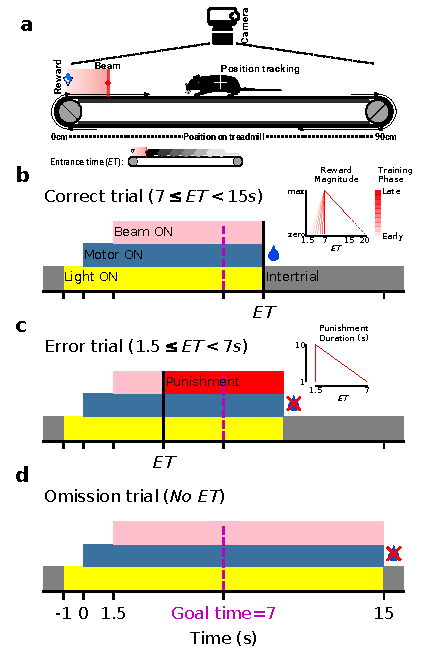
\includegraphics[scale=1]{ch-methods/figures/TaskRulesFULL.pdf}
    \caption[Treadmill Task Rules]
        {\textbf{Treadmill task and trial types.}
        \textbf{a)}
        Rats were enclosed on a powered treadmill.
        The infrared beam marked the reward area (red shaded area).
        During each trial, the belt pushed the animals away from the reward area and the first infrared beam interruption defined the \gls{et}.
        During trials and intertrials, the animal's position was tracked via a overhead video camera.
        \textbf{b)}
        Schematic description of a rewarded correct trial.
            \textit{Inset}: the magnitude of the delivered reward dropped linearly as \gls{et} increased (maximum reward at \acrlong{gt}).
            In early stages of training, smaller rewards were delivered for trials with ET~$<$~7~s.
            The smallest \gls{et} value that triggered reward delivery was progressively raised during learning.
        \textbf{c)}
        Schematic description of an error trial.
        Early \gls{et} triggered an extra running penalty and an audio noise.
            \textit{Inset}: the duration of the penalty was 10~s for the shortest \glspl{et} and fell linearly to 1~s for \glspl{et} approaching 7~s.
        \textbf{d)}
        Schematic description of an omission trial (no beam crossing between 1.5~s and 15~s).
        \textbf{b-d)}
        Note that \glspl{et} started to be detected 1.5~s after the motor start.
    }
    \label{fig:methods:taskRules}
\end{SCfigure}

\subsection{Habituation} \label{ch:methods:habituation}
Animals were handled 30~min per day for 3 days, then habituated to the treadmill for 3 to 5 daily sessions of 30~min, while the treadmill's motor remained turned off and a drop of reward was delivered every minute.
Habituation sessions resulted in systematic consumption of the reward upon delivery.

\subsection{Treadmill Task} \label{ch:methods:normalTrdTask}
Training started after handling and habituation sessions.
Each animal was trained once a day, 5 times a week (no training on weekends).
Each of the daily sessions lasted for 55~min and contained $\sim$130 trials.
Each trial started by turning the treadmill motor on at a fixed speed of 10~cm/s. 
One second before motor onset, the ambient light was turned on (to warn the animals of the imminence of the belt movement). 
The conveyor belt moved toward the rear of the treadmill (\Autoref{fig:methods:taskRules}{a}). 
Three types of trials were defined based on the time the animal first interrupted the infrared beam, i.e., the \gls{et}, relative to the \gls{gt}.
Trials in which animals entered the reward area after the \gls{gt} were classified as \emph{correct} ($7\leq ET<15$, \Autoref{fig:methods:taskRules}{b}).
Trials in which animals entered the reward area before the \gls{gt} were classified as \emph{error} ($1.5\leq ET<7$, \Autoref{fig:methods:taskRules}{c}).
In case no infrared beam interruptions were registered in 15~s, the trial ended and was classified as \emph{omission} (\Autoref{fig:methods:taskRules}{d}).
The infrared beam was inactive during the first 1.5~s ($ET<1.5$) to give the opportunity to the animals to leave (passively or actively) the reward area at the beginning of each trial.
Additionally, the exact value of the \gls{et} determined a reward/punishment ratio.
The reward was a drop of sucrose solution and the punishment was a period of extra running.
The running penalty started when the animals erroneously crossed the infrared detector before \gls{gt} (error trial) and its duration varied between 10~s and 1~s, according to the error magnitude (\Autoref{fig:methods:taskRules}{c, inset}).
Thus, to maximize reward collection and minimize running time, animals should cross the infrared beam just after the \gls{gt}.

\subsubsection{Reward Profile} \label{ch:methods:reward}
The magnitude of the reward was a function of the \gls{et} and animal's performance in previous sessions.
Reward was maximal at $ET=GT$ and dropped linearly to a minimum (i.e., $\sim 38\%$ of the maximum) for \glspl{et} approaching 15~s (maximum trial duration).
Moreover, in the beginning of the training, partial reward was also delivered for error trials with $ET>ET_0$, where $ET_0$ denotes the minimum threshold for getting a reward.
The magnitude of this additional reward increased linearly from zero for $ET=ET_0$, to its maximum volume for $ET=GT$.
In the first session of training, $ET_0=1.5$~s and for every following session, it was updated to the maximum value of median \glspl{et} of the past sessions.
Once $ET_0$ reached the \gls{gt}, it was not updated anymore (late training reward profile in \Autoref{fig:methods:taskRules}{b, inset}).

\subsection{Alternative Task Conditions}
In addition to the ``normal'' treadmill task described above, several modified versions of the task were also designed to investigate the embodiment hypothesis.
In each of these conditions, a specific parameter of the task was altered, allowing us to study its effect on animals' performance.

\subsubsection{Variable Speed Condition}
In this condition, for each trial, treadmill speed was pseudo-randomly drawn from a uniform distribution between 5 and 30~cm/s.
During any given trial, the speed remained constant.
We used 5~cm/s as the lowest treadmill speed, because lower speeds generated choppy movements of the conveyor belt.
Also, velocities higher than 30~cm/s were not used, to avoid any physical harm to the animals.

\subsubsection{No-timeout Condition}
In the control condition, the infrared beam was not active during the first 1.5~s of the trials. 
This \emph{timeout} period was sufficient to let the animals be carried out of the reward area by the treadmill, provided they did not move forward.
In the ``no-timeout'' condition, the infrared beam was activated as soon as the trial started.
Thus, in this condition, error trials corresponded to \glspl{et} between 0 and 7~s.
Consequently, animals were penalized if they were in the reward area when the trial started (i.e., $ET=0$~s).

\subsubsection{Short Goal Time Condition}
In this condition, the \gls{gt} was set to 3.5~s, half the value for the control condition.
The reward profile in this condition followed the same rules as for the control condition, except that reward was maximal at $ET=GT=3.5$~s.
Two different groups of animals were trained in this condition, one with treadmill speed set to the normal value of 10~cm/s, and another with treadmill running twice as fast.
In the short goal time condition, we also examined if the increased variability in \gls{et} could be attenuated when the penalty associated with early \gls{et} was increased and when reward magnitude was decreased for late \glspl{et}.
This was implemented by doubling the treadmill speed during the penalty period (from 10~cm/s to 20~cm/s), and the reward was delivered for a narrower window of \glspl{et} (maximal reward at $ET=GT=3.5$~s, and no reward after $ET=4.5$~s).
For proper comparison, we also examined the behavior of rats trained with $GT=7$~s when the running penalty was increased and the reward was decreased for late \glspl{et} (maximal reward at $ET=GT=7$~s, and no reward after $ET=9$~s).

\subsubsection{Immobile Condition}
In this condition, the treadmill motor was never turned on.
The ambient light was turned on during the trials and turned off during the intertrials.
Error trials were penalized by an audio noise and extended exposure to the ambient light.

\subsection{Reverse Treadmill Task} \label{ch:methods:rev}


\subsection{Locomotion Task} \label{ch:methods:loco}